\documentclass[]{article}

\usepackage{amsmath}
\usepackage{graphicx}
\usepackage{titlesec}
\usepackage{float}

%opening
\title{Calculating Phase Noise}
\author{}

\begin{document}

\maketitle



\section*{Initial Assumption}
In order to calculate the noise, I first assume the systematic error is near zero and strictly consider the data. I believe that the phase noise is produced by the fact that our interference pattern has some height due to random noise. This height causes and ambiguity when it comes to fitting a curve to the data. When the fitting minimizes the $\chi^2$ it snaps the fit to one edge of the data producing an error. Here I'll attempt to quantify that error. 
\section*{Calculation}
First, I calculate the height of our noise. This is done by consecutively opening small windows in the data and computing the difference between the min and max values and storing them if they are below some threshold. I use the threshold because I am only concerned about the height of the clean signal without looking at any flips or large noise at high gate voltages. The mean of the values is calculated for a single data set, and then the mean of all the means is calculated. For example, the June 5/2 data has a height of 0.0527 k$\Omega$.

Knowing the height of the data, we can now calculate the induced phase difference between the left and right edge of the data. It is simply,
\begin{eqnarray}
A\sin(\omega V_g) - A\sin(\omega V_g + \phi_{noise}) = \text{Singal Height} \\
\phi_{noise} = \sin^{-1}(\frac{Height}{A}) \approx \frac{Height}{A}
\end{eqnarray}

For rd9a from June 2014, we have $\phi_{noise} = \frac{0.0527}{0.154} = 0.342 = 0.11 \pi$.

\section*{In Practice}
Let us take a look at rd9a from the 2014 data set. Fig.~\ref{datasnap} shows a snapshot of the raw data.
\begin{figure}[H]
	\centering
	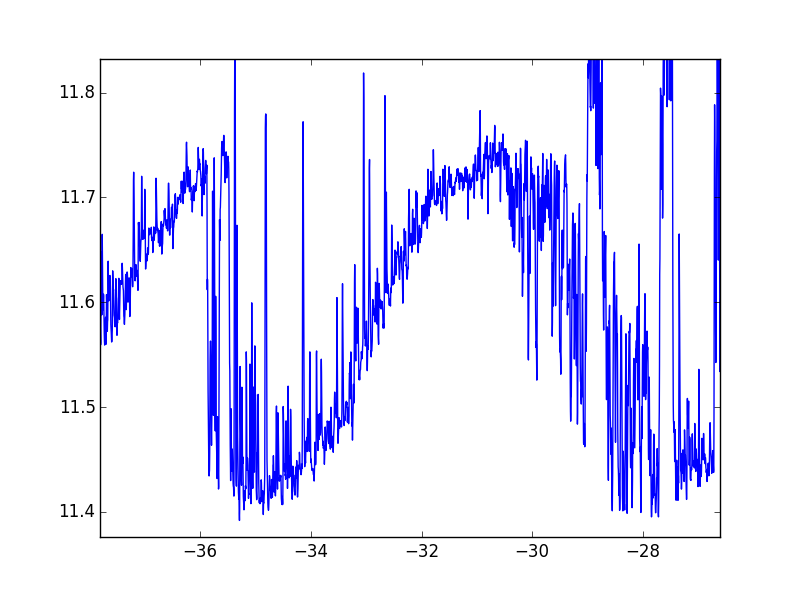
\includegraphics[width=8cm]{datasnap.png} 
	\caption{Snapshot of raw data}
	\label{datasnap}
\end{figure} 
Now, let us plot a line to the right edge of this data.
\begin{figure}[H]
	\centering
	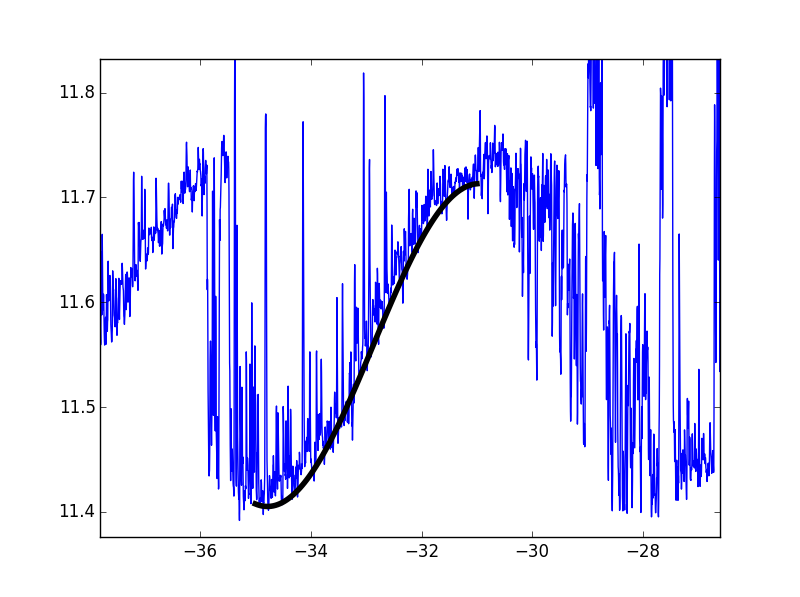
\includegraphics[width=8cm]{line1snap.png} 
	\caption{Curve fit to the right of the data}
	\label{line1snap}
\end{figure}
Using the $\phi$ value we calculated, let us plot a second line.
\begin{figure}[H]
	\centering
	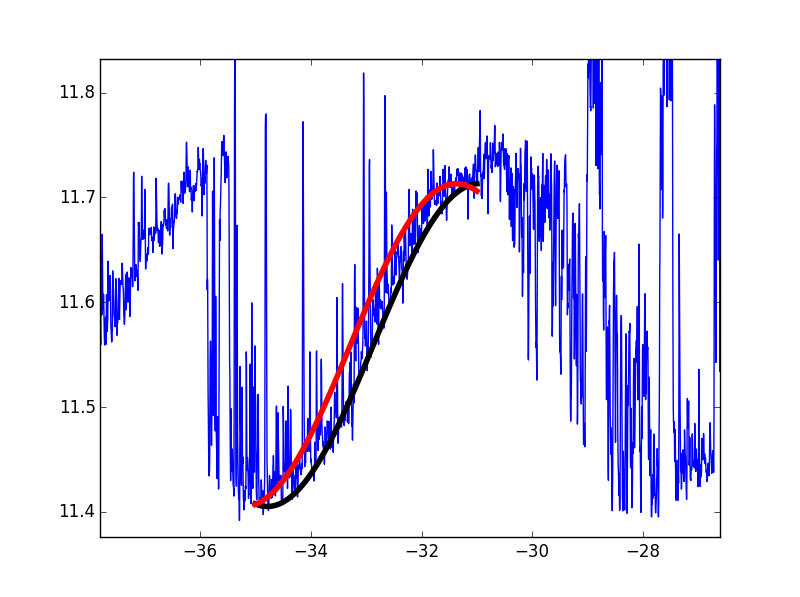
\includegraphics[width=8cm]{line2snap.png} 
	\caption{Left line plotted using calculated $\phi$ value}
	\label{line2snap}
\end{figure}
It seems that these two lines well define the data at the left and right boundaries, thus I believe that we can use this value of 0.11 $\pi$ as a noise width for our histograms.
\end{document}
